\section{Fitting lines to data  -- Practice exercises}

\begin{enumerate}
\item Noel is considering investing in a company's stock so he looked up a few values.
\begin{center}
\begin{tabular} {|l |c |c |c|} \hline
Day & 0 & 300 & 500 \\ \hline
Value (\$) & 23.19 & 37.00 & 48.10 \\ \hline
\end{tabular}
\end{center}
\begin{enumerate}
\item Calculate the rate at which the stock prices changed during the first 300 days. \vfill
\item Calculate the rate at which the stock prices changed from Day 300 to Day 500. \vfill
\item Is this growth linear? \bigskip
\item The scatter plot shows additional values of the stock Noel is considering buying.
\begin{center}
\scalebox {.9} {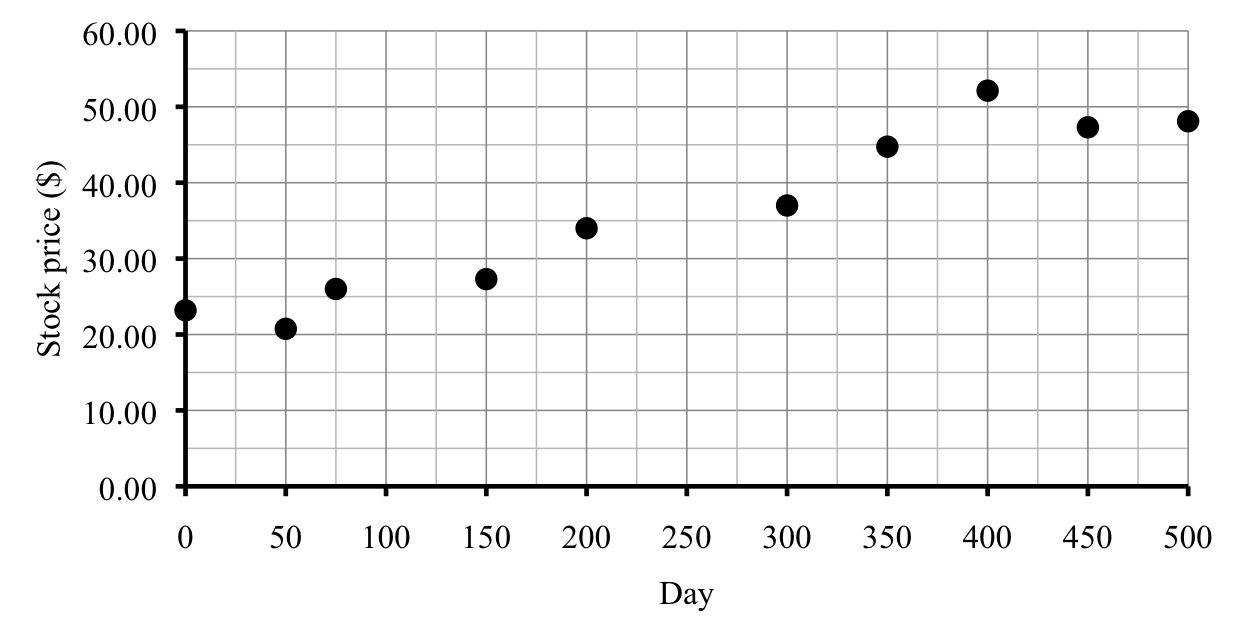
\includegraphics [width = 6in] {stockprices.png}}
\end{center}
\item Draw in a line that through the points for Day 300 and Day 500.  Label this line \#1.   Explain why that line does not fit the data well. \vfill
\item Draw in a line that fits the data better.  It does not need to go through any of the points exactly. Label that line \#2.  
\end{enumerate}

\newpage %%%%%%

\item Is it true that students who work part-time have lower grades?  Do the number of hours matter?  The table shows the grade point average (GPA) of ten students compared to the number of hours per week each student works at a part time job.  The variables we used are $H$ for the time worked at job (hours/week) and $G$ for the grades  GPA, on the usual scale of 0.0 to 4.0.
\begin{center}
\begin{tabular} {|c ||c |c |c |c |c |c |c |c |c |c|}\hline
$H$ & 0&0&10&12&14&15&16&18&20&20 \\ \hline
$G$ & 3.72 & 3.91 & 3.43 & 2.79 & 3.08 & 2.62 & 2.44 & 3.17 & 3.00 & 2.55 \\ \hline
\end{tabular}
\end{center}
\begin{enumerate}
\item Make a scatter plot of the points.  Start the $G$-axis at 2.0.
\begin{center}
\scalebox {.8} {
\includegraphics [width = 6in] {GraphPaper.jpg}}
\end{center}
\bigskip

\item Find the equation of the line that goes through the first and last point listed.

\emph{Hint:  the first point tells you the intercept.}  \vfill \vfill
\item Draw this line on your graph and label it line A. 

\newpage %%%%%%
~\hspace{-.5in} \emph{The problem continues \ldots}

\item Use your equation for line A to figure out what you would expect the GPA of a student working a 30 hour per week job to be. \vfill
\item It turns out, the best fitting line has equation $G=3.7597-.0551H$.  Make a table of values for this equation using $H=0, 10, 20$ hours.  \vfill \vfill
\item Use that table of values to graph this best fitting line on that same set of axes.  Label it line B.  \bigskip
\item According to line B, what's the most hours a student should work to be able to maintain a 3.5 GPA?  Solve an equation, then check on your graph. \vfill \vfill
\end{enumerate}

\newpage %%%%%%

\item Mia and Mandi and opened a candy shop this January.  The table shows their monthly sales profit.  Except for some seasonal fluctuation, Mia and Mandi generally expect your profits to rise steadily while their business is getting established.  
\begin{center}
\begin{tabular} {|c||c|c|c |c|c|c|c|c|}  \hline
Month & Jan & Feb & Mar & Apr & May & Jun & Jul  & Aug \\ \hline
Sales Profit (\$) & \text{3,394} & \text{4,702} & \text{3,683}  & \text{4,840}  & \text{5,632}  & \text{4,432}  & \text{4,649}&  \text{4,590} 
 \\ \hline
\end{tabular}
\end{center}
\begin{enumerate}
\item Make a scatter plot.  Begin the profit axis at \$\text{3,000}.
\begin{center}
\scalebox {.8} {
\includegraphics [width = 6in] {GraphPaper.jpg}}
\end{center}
\bigskip
\item Name the variables and write an equation for the line through January and August.  Add this line (\#1) to your graph.  This line is too low. \vfill \vfill

\newpage %%%%%%
~\hspace{-.5in} \emph{The problem continues \ldots}

\item Write an equation for the line through March and July.  Notice that you need to find the intercept this time.  Add this line (\#2) to your graph.  This line is too steep. \vfill \vfill \vfill
\item Neither of these lines go anywhere near the data for February, April, and May, because those are outliers.  Any idea why those months had much higher candy sales than the other months? \vfill
\item What does each equation give as an estimate for September's sales?  \vfill
\item Explain why Mia and Mandi should not use either of these lines to estimate October's sales. \vfill
\end{enumerate}

\newpage %%%%%%

\item The scatter plot shows the total volume of wood, $V$ cubic feet,  in managed forests of different ages, $A$ years.
For each line, decide if it's a good fit or not.  Explain.  

\begin{center}
\begin{tabular} {lcl}
LINE A & &LINE B \\ 
 \scalebox {.4} {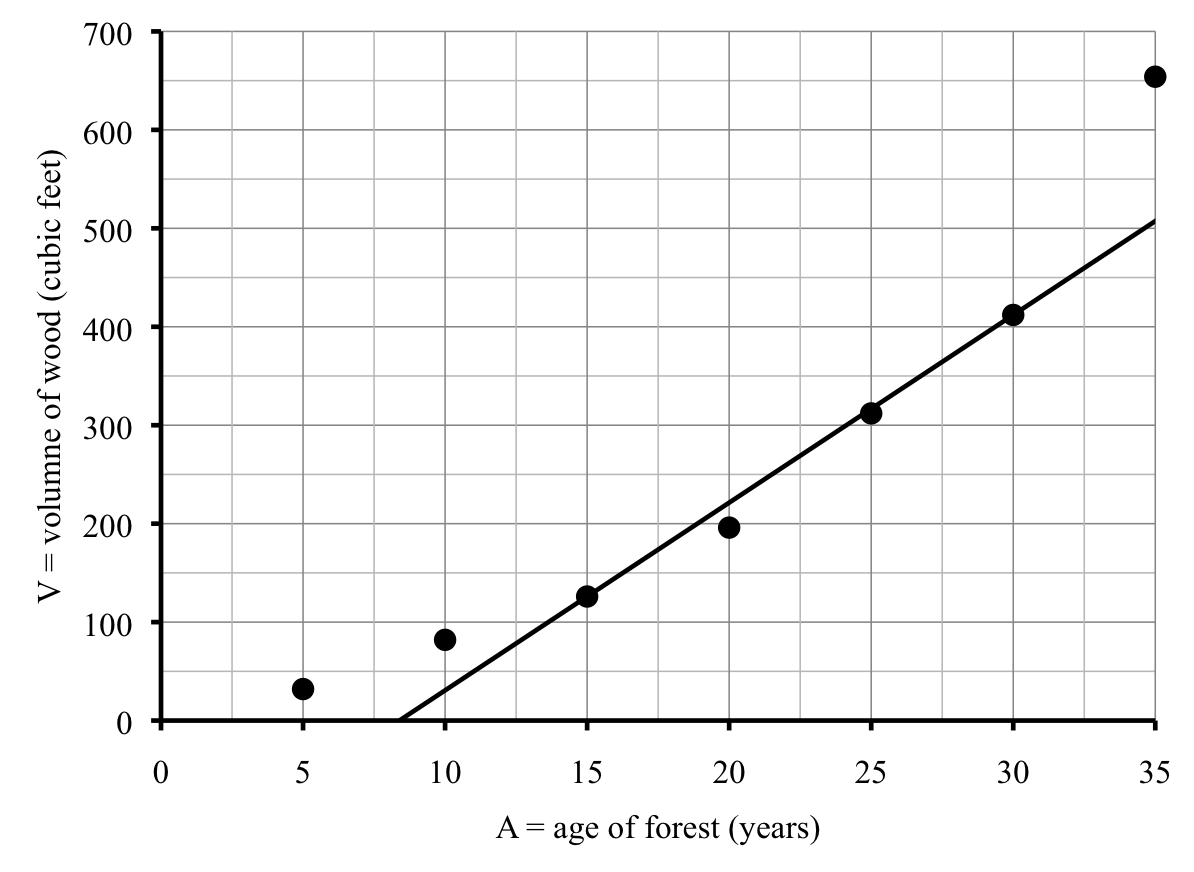
\includegraphics [width = 6in] {woodforestA.png}} 
& ~\hspace{.45in} &
 \scalebox {.4} {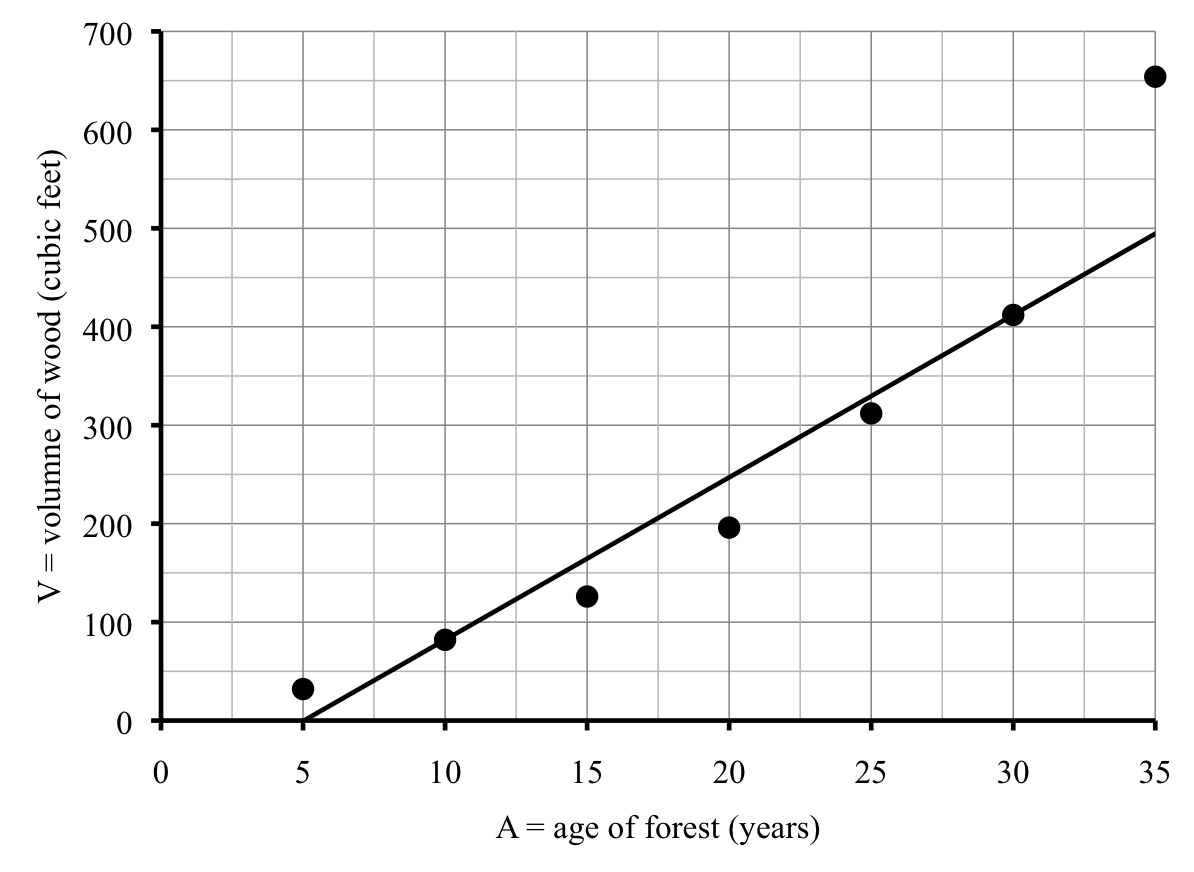
\includegraphics [width = 6in] {woodforestC.png}} \\
\end{tabular}
\end{center}

\vfill

\begin{center}
\begin{tabular} {lcl}
LINE C & & LINE D \\
 \scalebox {.4} {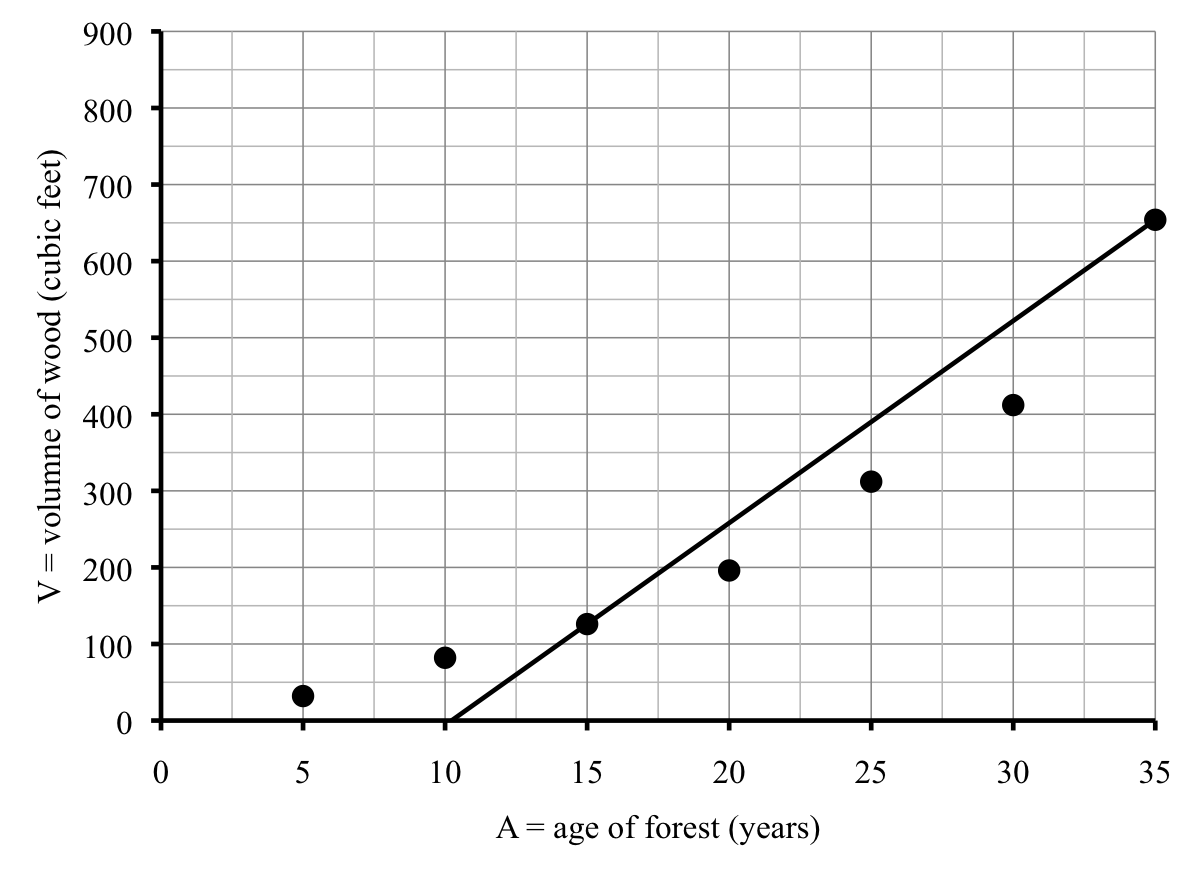
\includegraphics [width = 6in] {woodforestD.png}}
& ~\hspace{.45in} &
 \scalebox {.4} {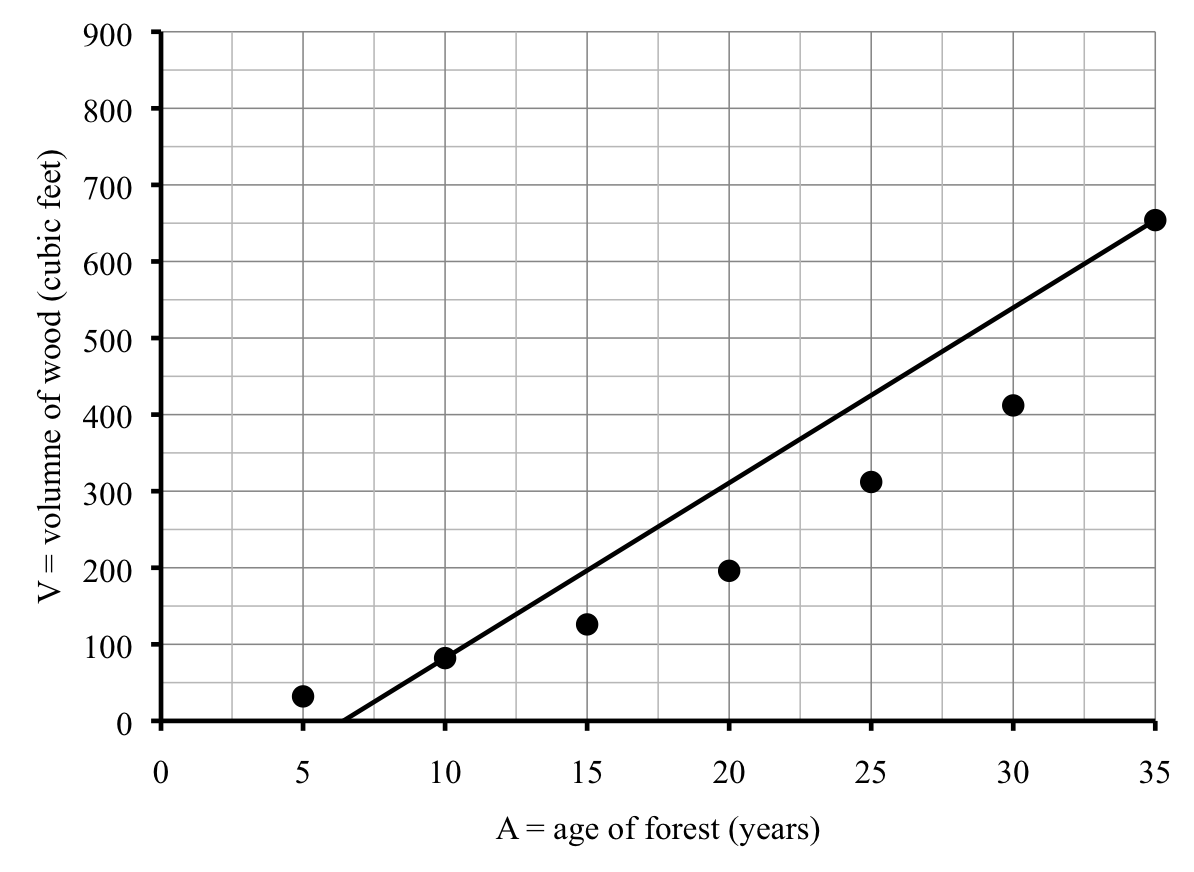
\includegraphics [width = 6in] {woodforestE.png}} \\ 
\end{tabular}
\end{center}
\vfill
 
 

%LINE A \\
% \scalebox {.4} {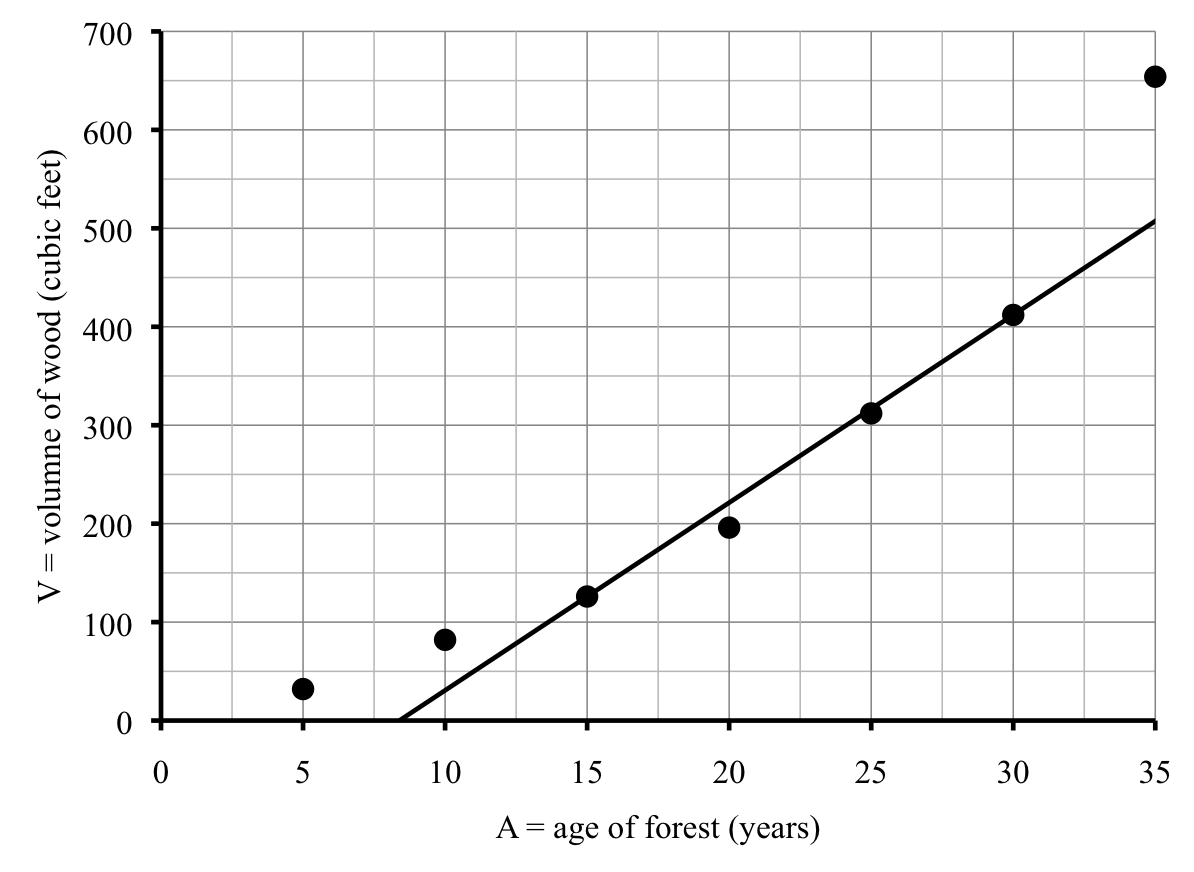
\includegraphics [width = 6in] {woodforestA.png}} 
% 
%LINE B \\
% \scalebox {.4} {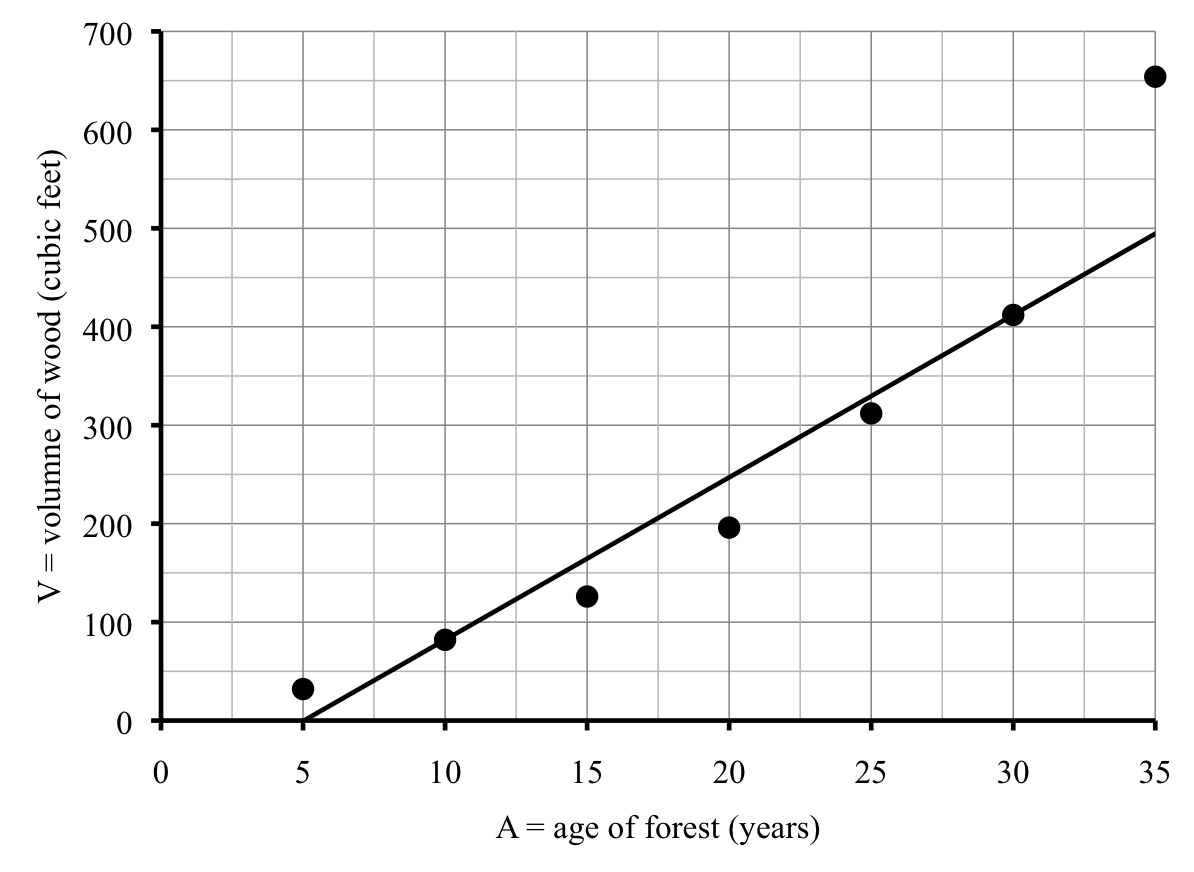
\includegraphics [width = 6in] {woodforestC.png}}

%LINE C \\
% \scalebox {.4} {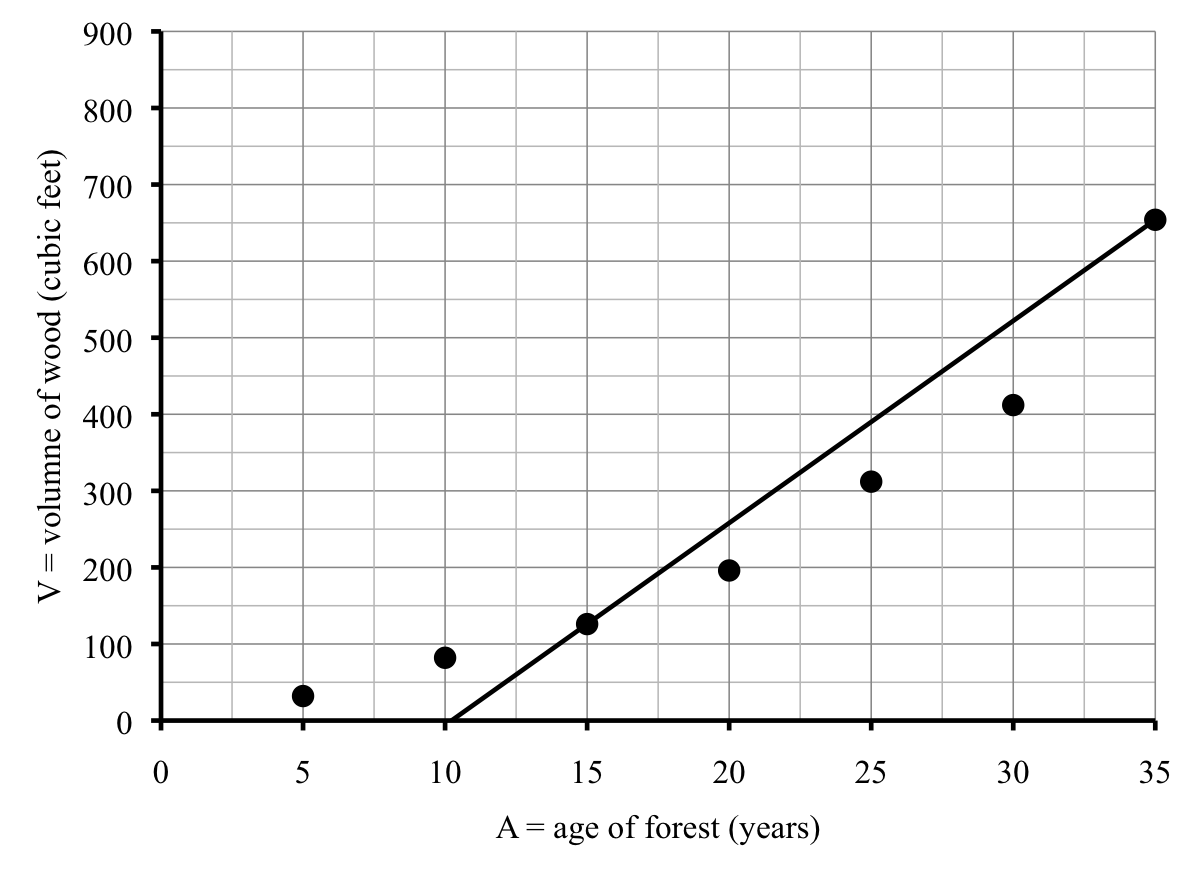
\includegraphics [width = 6in] {woodforestD.png}}
% 
%LINE D \\
% \scalebox {.4} {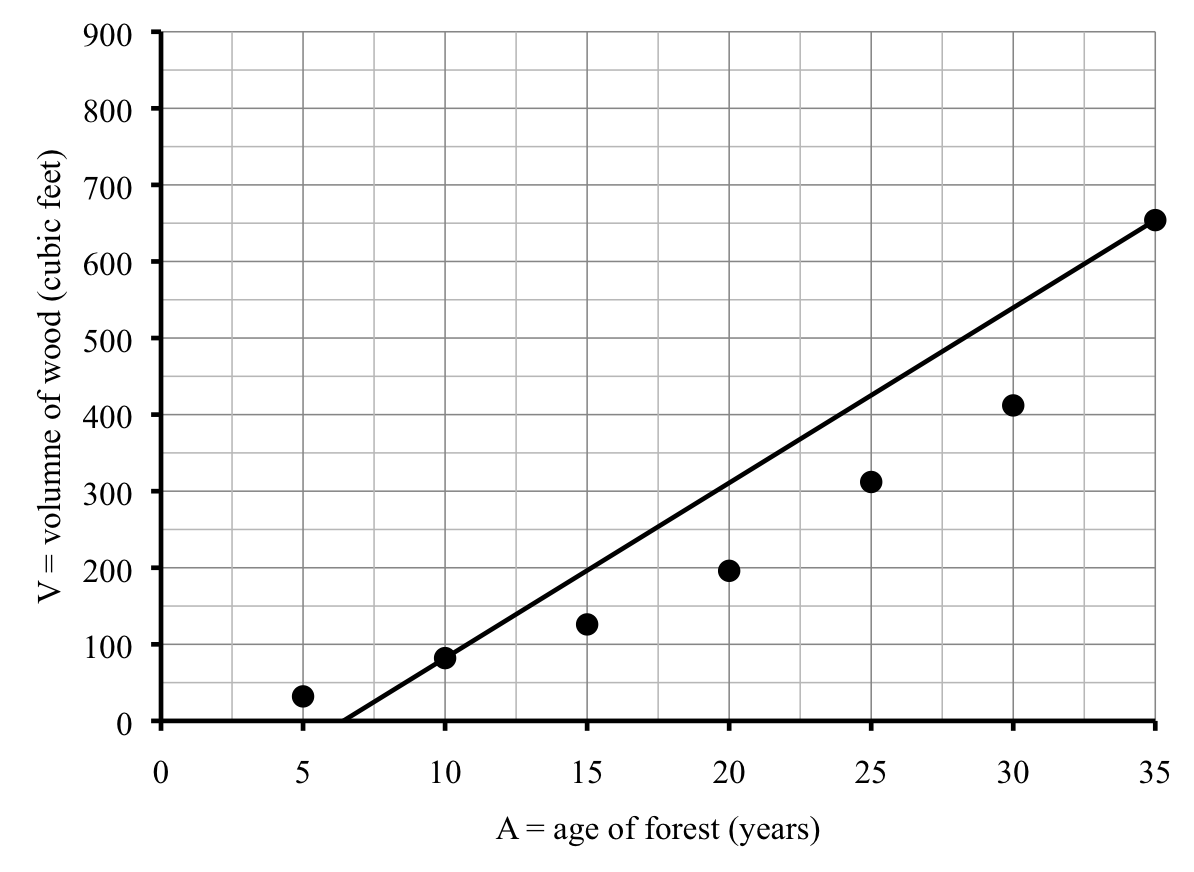
\includegraphics [width = 6in] {woodforestE.png}}
%%%%%%

%\item The following table shows the total volume of wood, $V$ cubic feet,  in managed forests of different ages, $A$ years.
%\begin{center} 
%\begin{tabular} { |c| |c |c |c |c |c |c |c|} \hline
%$A$ & 5 & 10 & 15 & 20 & 25 & 30 & 35 \\ \hline
%$V$ & 32 & 82 & 126 & 196 & 312 & 412 & 654 \\ \hline
%\end{tabular}
%\end{center}
%For each line drawn, decide if it's a good fit or not.  If not, explain why.
%\bigskip

\end{enumerate}
